\documentclass[12pt,letterpaper]{article}


\newcommand{\studentname}{Ben Bassett}

\title{\textsc{Lab 09: Ray Optics with Lenses}}
\newcommand{\shorttitle}{Ray Optics with Lenses}

\newcommand{\course}{PHY310}
\newcommand{\labdate}{11-5-2024}

%------------------------------------------------------------------------------------------------------------

\usepackage[letterpaper,left=1in,right=1in,bottom=1in,top=1in]{geometry}
\usepackage{fancyhdr}
\usepackage{subfigure}
\usepackage{graphicx}
\usepackage{amsmath}
\usepackage{cleveref}
\usepackage{booktabs}
\usepackage[british]{babel}
\usepackage[square,comma,numbers,sort&compress]{natbib}
\usepackage{csvsimple}
\usepackage{graphicx}
\usepackage{pgfplotstable}
\usepackage{textcomp,gensymb}
\usepackage{array}
\usepackage{tabu}
\usepackage{multirow}
\usepackage{url}
\usepackage{lipsum}
\usepackage{dsfont}
\pgfplotsset{compat=1.9}% supress warning
\begin{document}

%------------------------------------------------------------------------------------------------------------

\setlength{\parindent}{1em}
\setlength{\parskip}{0.5em}
\author{\course~Lab Journal \\ \\ \studentname} % \,\& \labpartner}
\date{\labdate}

\renewcommand\abstractname{Summary}

\pagestyle{fancy}
\fancyhead{}
\fancyhead[l]{\course:~\shorttitle}
\fancyhead[r]{\studentname}
\fancyfoot{}
\fancyfoot[C]{\thepage}
\renewcommand{\headrulewidth}{0pt}
\renewcommand{\footrulewidth}{0pt}

\renewcommand\bibname{References}

%------------------------------------------------------------------------------------------------------------

\renewcommand\abstractname{Abstract}
\maketitle

% COMMENT IN IF ASKED TO SUBMIT REPORT WITH ABSTRACT
\begin{abstract}
In this lab we used the magnific properties of lenses to measure something small on a scale we could more easily work with. Knowing the focal lengths of the lenses and distances between them we were able to compute the total magnification using the thin lens equation and find the original distance from the value we measured when magnified.
\end{abstract}

\section{Experimental Apparatus}

Materials given were an optics track, incandescent light source, a white plate, a ruler, and an assortment of lenses. Our setup is illustrated in Figure \ref{fig:setup}.

\begin{figure}[h]
    \centering
    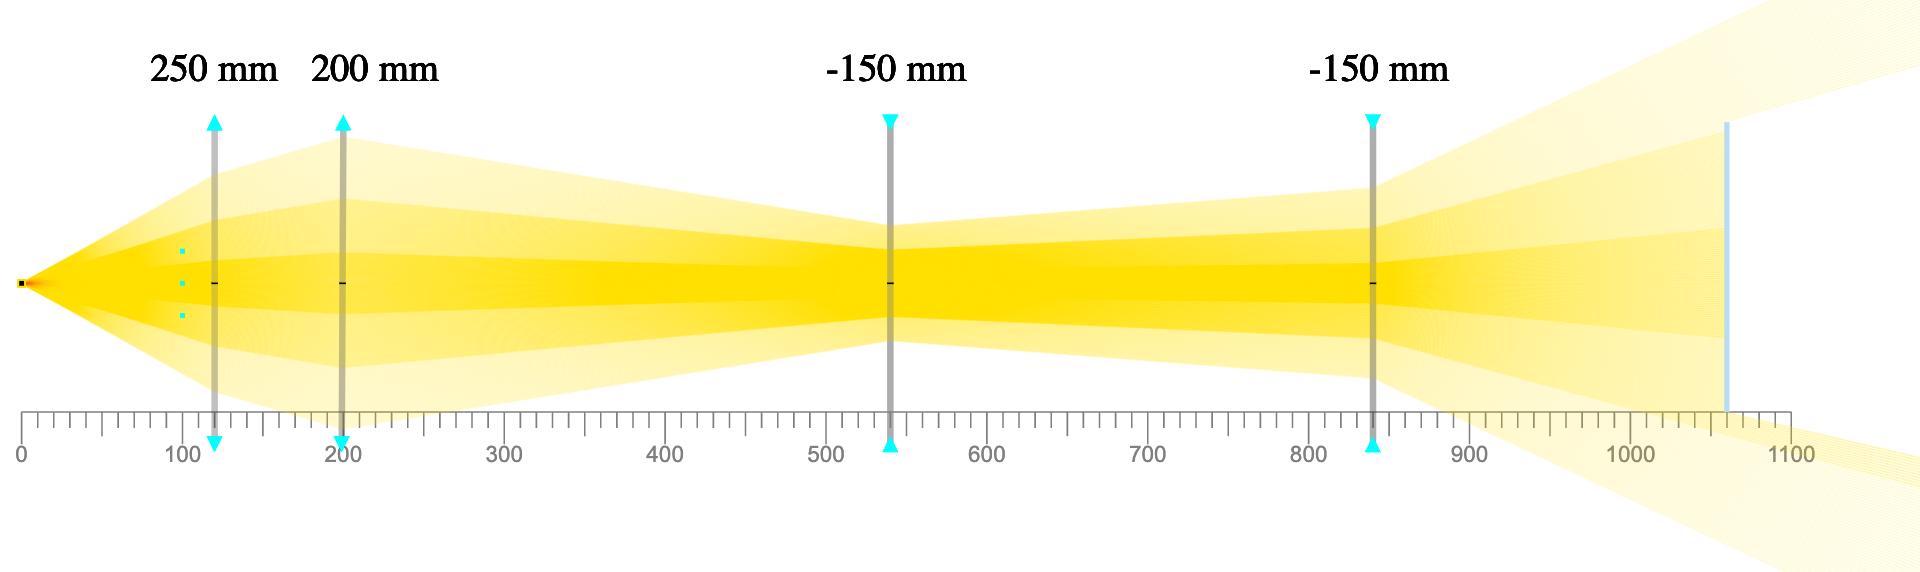
\includegraphics[width=6in]{images/setup.png}
    \caption{The final optics track setup}
    \label{fig:setup}
\end{figure}

% \pagebreak
\section{Procedure}

After much tinkering, we setup our lenses in the following sequence:

\begin{itemize}
    \item 250 mm lens at 12 cm
    \item 200 mm lens at 20 cm
    \item -150 mm lens at 54 cm
    \item -150 mm lens at 84 cm
\end{itemize}

Our light source was obviously at 0 cm, and our projection plate was at 106 cm. We used our ruler to measure across our in-focus image to get the magnified diameter of the filament.

\section{Results}

We used the thin lens equation to compute the magnification

\begin{equation}
\frac{1}{f} = \frac{1}{d_o} + \frac{1}{d_i}
\end{equation}

where $f$ is the focal length of the lens, $d_o$ is the object distance, and $d_i$ is the image distance. Then for each lens, the magnification $M$ is given by:

\begin{equation}
m = -\frac{d_i}{d_o}
\end{equation}

Let's compute this for each lens, then multiply them to get the total magnification!

\begin{table}[h]
\centering
\begin{tabular}{|c|c|c|c|c|}
\hline
Lens & Position (cm) & Focal Length (mm) & Image Distance (cm) & Magnification \\
\hline
1 & 12.0 ± 0.1 & 250 & -23.077 ± 0.370 & 1.923 ± 0.035 \\
2 & 20.0 ± 0.1 & 200 & 56.111 ± 1.249 & -1.806 ± 0.046 \\
3 & 54.0 ± 0.1 & -150 & -46.641 ± 5.575 & -2.109 ± 0.279 \\
4 & 84.0 ± 0.1 & -150 & -12.545 ± 0.149 & 0.164 ± 0.012 \\

\hline
\multicolumn{4}{|c|}{Total Magnification} & 7.324 ± 0.995 \\

\hline
\multicolumn{4}{|c|}{Final Image Distance (cm)} & 98.641 ± 5.576 \\

\hline
\end{tabular}
\caption{Lens positions, focal lengths, image distances, and magnifications}
\label{tab:lens_system}
\end{table}


All of our data and computation is in Table 1. On our final image, we measured the diameter of the magnified filament coils to be 20 mm in diameter, which means that given our magnification of $\mathbf{7.32 \pm 0.99}$, the actual diameter of the filament coils should be $\mathbf{2.73 \pm 0.04} \textbf{ mm}$.

\section{Conclusions}

Our computation of the final filament diameter as $\mathbf{2.73 \pm 0.04} \textbf{ mm}$ seems reasonable, which seems like we did our magnification math properly. Success!

% \bibliographystyle{unsrtnat}
% \bibliography{references}

\end{document}
